\renewcommand*{\arraystretch}{1.5}
\begin{tabularx}{15cm}{|p{2.1cm}@{\hskip 1ex}|@{\hskip 1ex}X|}
	\hline
	number      & 9                                                          \\ \hline
	title       & Forum with related Tags                                                           \\ \hline
	\multicolumn{2}{|c|}{ 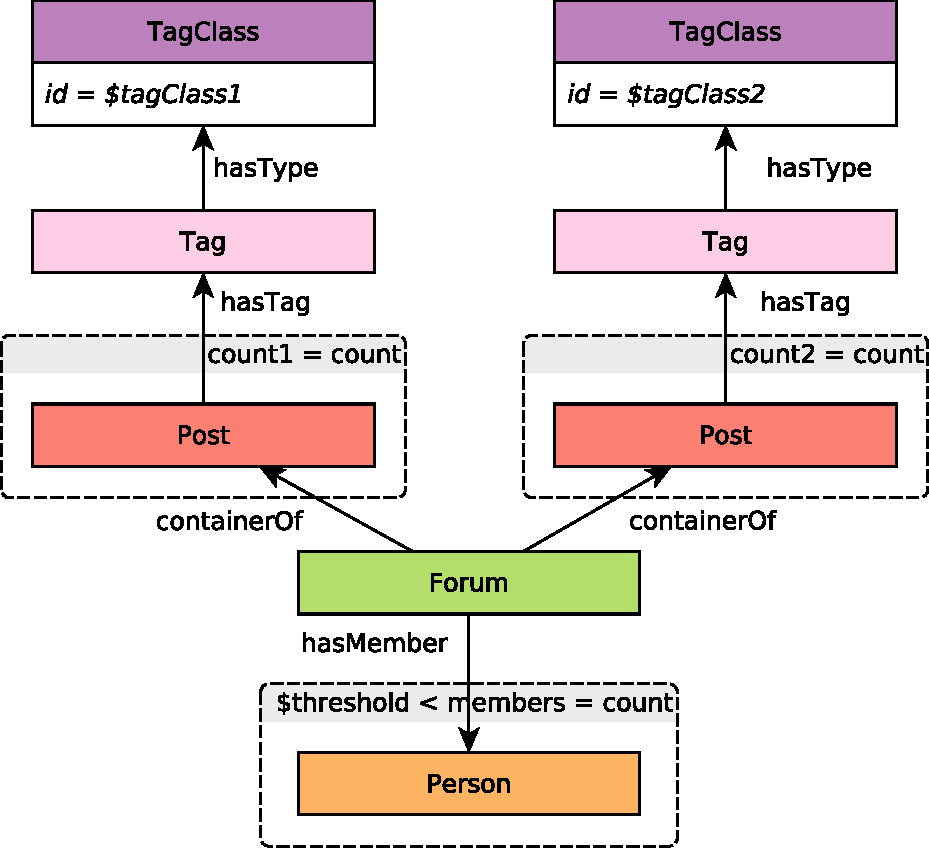
\includegraphics[scale=\patternscale,margin=0cm .2cm]{patterns/q09}} \\ \hline
	description & Given two TagClasses (\texttt{tagClass1} \& \texttt{tagClass2}), find
Forums that contain at least one Post with a Tag from \texttt{tagClass1}
and at least one Post with a Tag from \texttt{tagClass2} (direct
children not transitive) -- this may be the same Post.

Consider the Forums with a number of members greater than a given
threshold. For every such forum, count the number of Posts that have a
Tag from TagClass1 (count1), and the number of posts that have a tag
from TagClass2.
 \\ \hline
	
	parameters  &
	\multicolumn{1}{>{\raggedright}X|}{
		\variable{tagClass1}{32bitInteger} \\
		\variable{tagClass2}{32bitInteger} \\
		\variable{threshold}{32bitInteger} 
		}\\ \hline
	result      &
	\multicolumn{1}{>{\raggedright}X|}{
		\variable{forum.id}{64bitInteger}\\
		\variable{count1}{32bitInteger}Number of Posts with at least one tag belonging to tagClass1\\
		\variable{count2}{32bitInteger}Number of Posts with at least one tag belonging to tagClass2
		}\\ \hline
	sort        &
	\multicolumn{1}{>{\raggedright}X|}{
		\sortentry{count2}{\desc}\\
		\sortentry{count1}{\desc}\\
		\sortentry{forum.id}{\asc}
		}\\ \hline
	limit       & 100                                                           \\ \hline
	choke points        &
	\multicolumn{1}{>{\raggedright}X|}{
		\chokepoint{1.2}, 
		\chokepoint{1.4}, 
		\chokepoint{2.1}, 
		\chokepoint{2.3}, 
		\chokepoint{2.4}
		}\\ \hline
\end{tabularx}
\clearpage
